\section{教師の構成}
\label{sec_teacher}
本章では，教師ラベルを付ける Qwen3-VL-8B への指示の方法を検討した結果を述べる．
以下では，VLM に与える指示文をプロンプトと呼び，1回の推論で1つのプロンプトを与えることを1つの質問と呼ぶ．
教師は，1枚の画像に複数の質問をし，その回答を規則で組み合わせる構成とした．

\subsection{推論の条件}
全ての質問は，Qwen3-VL-8B-Instruct を量子化せずに vLLM で実行した．
入力画像は1枚とし，最大画素数を $ 448 \times 448 $ に制限した．
生成は温度0の貪欲生成とし，出力は JSON スキーマによる構造化出力でラベルの候補に制約した．
入力の最大画素数を $ 256 \times 256 $ に下げると速度は約1.4倍になったが，正解率は 0.905 から 0.880 に低下した．
小さな空欄や文字の判読に解像度が必要なためと考えられる．
一方，$ 672 \times 672 $ に上げても形式の正解率の改善は0.6ポイントにとどまり，速度は半分になった．

\subsection{最終の教師の質問}
表\ref{tab_questions}に，最終の教師を構成する質問を示す．
表の名称は本稿での呼び名であり，括弧内は実装での識別子である．
実装の識別子は，プログラムと実験の記録との対応を示すために併記する．

\begin{table*}[t]
    \centering
    \caption{最終の教師を構成する質問}
    \label{tab_questions}
    \small
    \begin{tabular}{>{\raggedright\arraybackslash}p{0.2\textwidth}>{\raggedright\arraybackslash}p{0.42\textwidth}>{\raggedright\arraybackslash}p{0.3\textwidth}}
        \toprule
        質問の名称 & 内容 & 用い方 \\
        \midrule
        形式の質問（F\_v2） & 形式と画風を問う短い英語のプロンプト．text は「画像のほぼ全体が文章で，主となる写真や絵がない」と定義する & 形式の回答のみ用いる．text はお題文に読み替える \\
        お題文の確認（O\_v10\_en） & 投稿者が回答者に向けて書いた問い，指示，題目の句があるかを英語で問う & 形式の質問がお題文とした画像のみ．偽なら通常にする \\
        属性の質問（J\_v6） & 属性，形式，媒体を日本語で一括して問う．属性を先に出力させる & 属性の回答のみ用いる \\
        文字の質問（X\_v10\_en） & ロゴや透かしを含め，読める文字があるかを英語で問う & カルタ記号のない画像に限り，属性の質問の文字ありと論理和をとる \\
        媒体の質問（M\_v6） & 媒体のみを日本語で問う & CG の回答は削除し，媒体が空ならイラスト \\
        絵画の質問（P\_v8\_en） & 画家が描いた美術作品であるかを英語で問う & 媒体の絵画をこの回答で置き換える \\
        \bottomrule
    \end{tabular}
\end{table*}

回答を組み合わせた後に，次の規則を適用する．
第1に，形式から属性を導き，カルタならカルタ記号あり，穴埋めなら空欄あり，お題文なら文字ありとする．
第2に，媒体が1つも選ばれていない場合はイラストとする．
第3に，形式がカルタの画像は，ボケの書き出しで照合する．
かなで始まるボケが5件以上あり，そのうち VLM が読み取った記号のひらがなで始まる割合が3割未満であれば，カルタではないとみなす．
この規則は，空欄の前後のひらがなや中身が空の枠を，VLM がカルタの記号と誤る事例を減らすために導入し，教師のカルタの F1 を 0.77 から 0.88 に向上させた．

\subsection{質問の分け方}
表\ref{tab_split}に，質問の分け方を変えた教師の通常の評価用データ640枚での精度を示す．
1行目は事前知識を含む第1版の定義，それ以外は第2版の定義での値である．

\begin{table}[t]
    \centering
    \caption{質問の分け方と教師の精度（評価用データ640枚）}
    \label{tab_split}
    \small
    \begin{tabular}{>{\raggedright\arraybackslash}p{0.42\linewidth}ccc}
        \toprule
        構成 & 形式の正解率 & 属性 & 媒体 \\
        \midrule
        4軸を一括 & 0.850 & 0.707 & 0.769 \\
        3軸を一括 & 0.902 & 0.773 & 0.761 \\
        形式のみ分割 & 0.923 & 0.799 & 0.761 \\
        形式と媒体を分割 & 0.923 & 0.799 & 0.835 \\
        \bottomrule
    \end{tabular}
\end{table}

表\ref{tab_split}の属性と媒体の列はマクロ F1 である．
全ての軸を1つのプロンプトで問うと，出力が約150トークンに増え，個々の判断の精度が下がった．
形式は短いプロンプトで単独に問うと最も正確であり，媒体も媒体のみを問う方が一括で問うより高かった．
一方，属性は属性のみを問うより，形式と媒体の定義を含めて一括で問う方が高かった．
属性の判定には，形式の判定手順の文脈が役立つと考えられる．
質問を分けると推論の回数は増えるが，教師は数万枚にラベルを付けるのみであるため，全体の費用への影響は小さい．

\subsection{形式の質問の改訂の試み}
最も正確であった形式の質問は，初期の7クラスのために書いたプロンプトであり，text の定義は第2版以降のお題文の定義と一致しない．
そこで，定義を一致させる改訂を複数試みた．
表\ref{tab_format_prompt}に，dev における形式の正解率を示す．

\begin{table}[t]
    \centering
    \caption{形式の質問の改訂の試み（dev の形式の正解率）}
    \label{tab_format_prompt}
    \small
    \begin{tabular}{>{\raggedright\arraybackslash}p{0.7\linewidth}c}
        \toprule
        形式の質問 & 正解率 \\
        \midrule
        元の短い英語のプロンプト & 0.944 \\
        定義書の文言で書いた日本語のプロンプト & 0.894 \\
        同上，入力を $ 672 \times 672 $ 画素に拡大 & 0.900 \\
        同上，文字とその出所を先に書き出させる & 0.828 \\
        元のプロンプトの text を「絵があってもよい」に変更 & 0.487 \\
        同上，「多くの画像は該当しない」を追加 & 0.412 \\
        元のプロンプトに，テンプレートの問いの文の例を追加 & 0.881 \\
        \bottomrule
    \end{tabular}
\end{table}

いずれの改訂も元のプロンプトを超えなかった．
text の定義に「絵があってもよい」を加えると，標識や漫画の台詞だけでなく，文字のほとんどない人物の写真までお題文と判定した．
「画像のほぼ全体が文章」という見た目の基準は，定義書とは一致しないが VLM にとって判定しやすく，その基準を失うと判定の手がかりがなくなると考えられる．
画像中の文字とその出所を先に書き出させる方法も，途中の判断の誤りが形式の誤りにつながり，精度を下げた．
定義との不一致による実際の損失は，評価用データで2枚程度であったため，形式の質問は元のプロンプトを据え置いた．

\subsection{お題文の過検出への対策}
形式の質問の主な誤りは，看板，歌詞，報道の画面，図表など，画像に元からある文字が多い画像をお題文とする過検出であった．
この対策として，次の2通りを比較した．
1つ目は，形式の質問のお題文または通常の説明に「看板，字幕，歌詞，図表など元からある文字は大きくてもお題文ではない」を書き足す方法である．
2つ目は，形式の質問は変えず，お題文と判定した画像に限り，投稿者が回答者に向けて書いた文があるかを別の短い質問で確かめる方法である．
以下では，2つ目の質問を確認の質問と呼ぶ．

実データの目視ラベル380枚において，元の構成ではお題文の誤検出が13件であった．
説明をお題文の側に書き足すと誤検出は18件から19件に増え，通常の側に書き足すと10件に減った．
確認の質問を用いると誤検出は4件に減り，見落としは2件から3件に増えるのみであった．
教師のお題文の F1 は，実データで 0.769 から 0.873，通常の評価用データで 0.810 から 0.879 に向上した．
図\ref{fig_odaibun_verify}に，確認の質問でお題文から通常に戻した画像の例を示す．
各画像の上に，お題 ID と目視の形式を示す．
戻した32枚のうち27枚は目視でもお題文ではなく，看板，選挙のカード，歌詞，答案，報道の画面などであった．

\begin{figure*}[t]
    \centering
    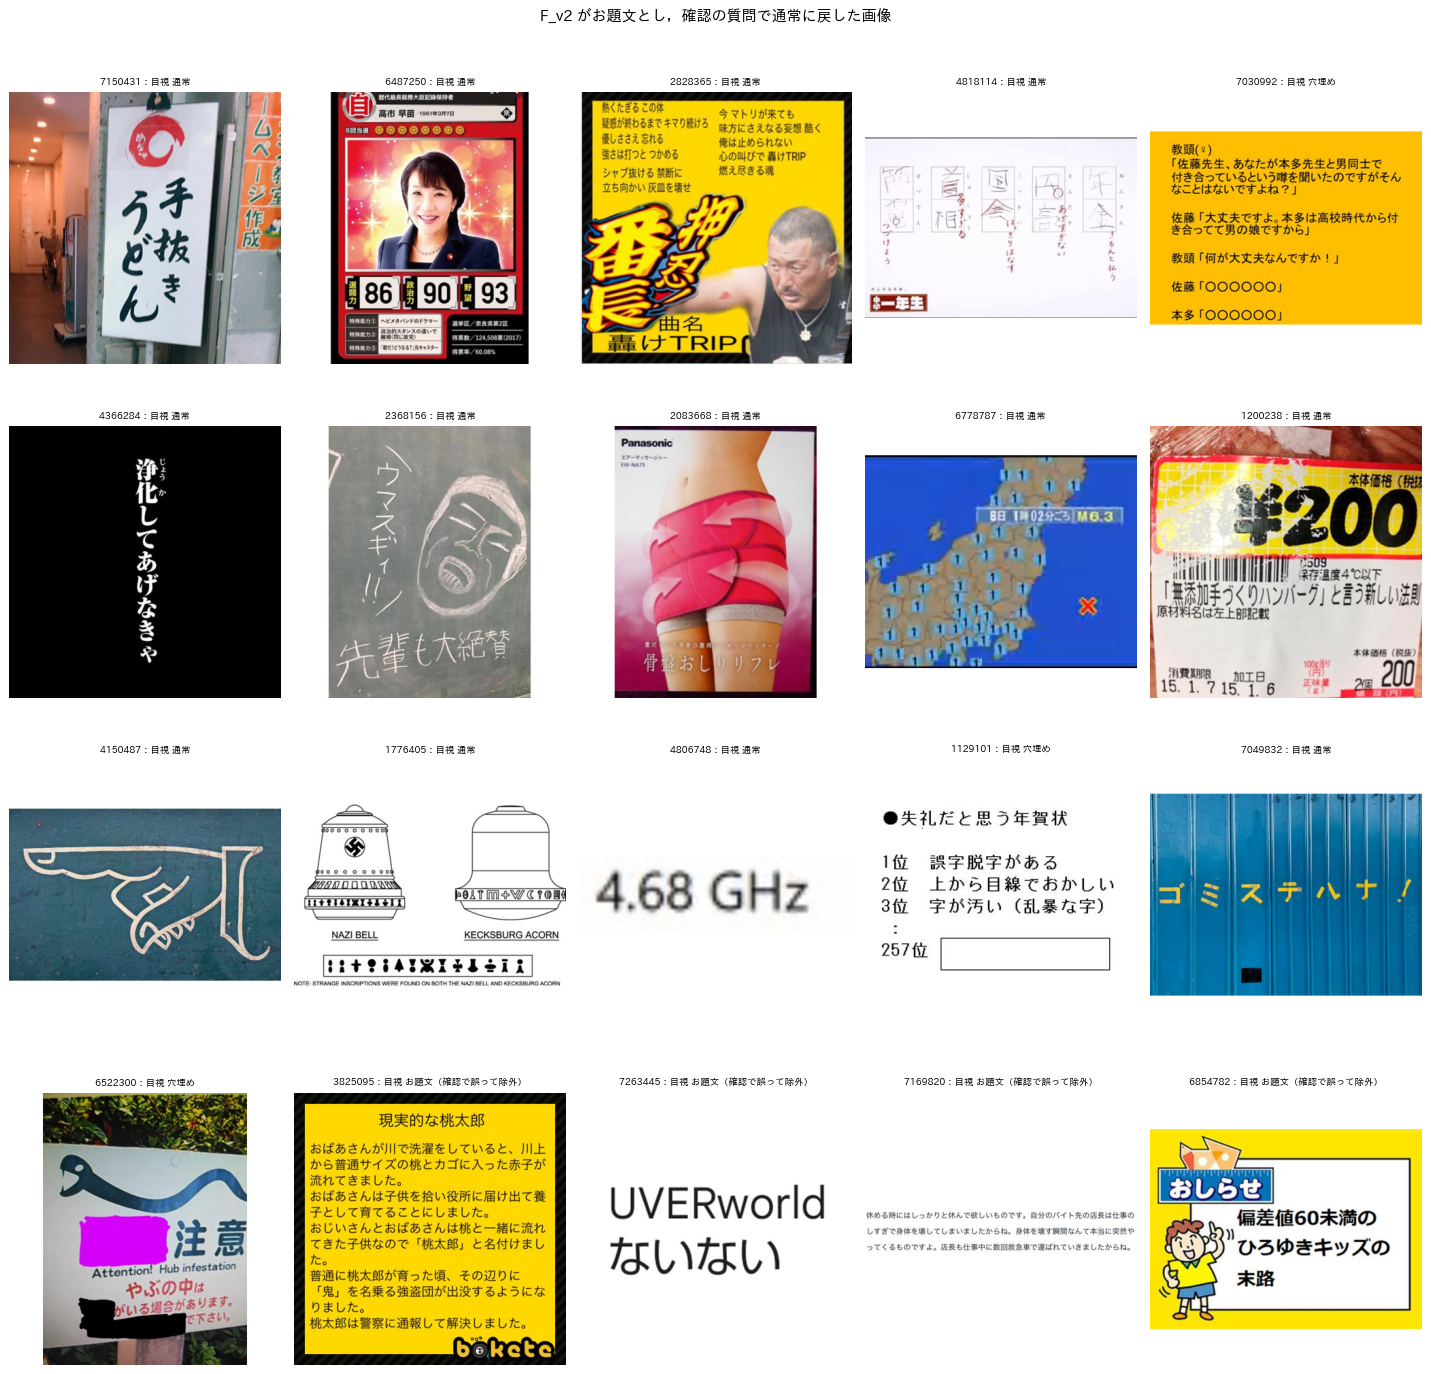
\includegraphics[width=0.8\textwidth]{figures/fig_odaibun_verify.png}
    \caption{形式の質問がお題文と判定し，確認の質問で通常に戻した画像の例}
    \label{fig_odaibun_verify}
\end{figure*}

同じ傾向は他の改訂でも見られた．
合成画像を「境界線で区切られた別々の写真の枚数」として問う質問や，お題文の位置と体裁を問う補助の質問は，いずれも適合率を下げた．
VLM は，テロップの帯やワイプの小窓を別々の写真と数え，テロップを投稿者が書き加えた文と判定した．
一方，絵画を独立の質問にすると，少ない区分の評価用データにおける教師の4区分の F1 の平均は，dev で 0.604 から 0.658，test で 0.591 から 0.715 に向上した．
媒体の質問では選択肢の多さに埋もれていた絵画が，独立の質問で見落とされにくくなったと考えられる．
これらの結果から，見た目で区別しにくい概念を問い方の工夫で判定させることは難しく，見た目の特徴がはっきりした概念や，誤りの多いクラスに対象を絞った確認の質問は有効であるといえる．

\subsection{文字ありの質問}
第4版の文字ありはロゴや透かしを含むが，属性の質問は旧定義に従ってこれらを除くよう指示していた．
そこで，読める文字があるかを独立に問う文字の質問を加えた．
文字の質問はほぼ見落としがない一方で，カルタの記号のひらがなだけの画像も文字ありと答えた．
そこで，カルタ記号のない画像に限り，文字の質問の回答と属性の質問の回答の論理和をとった．
これにより，教師の文字ありの F1 は実データで 0.954 から 0.971 に向上した．

\subsection{英語と日本語}
プロンプトの言語の影響を，属性の質問と絵画の質問で比較した．
英語版と日本語版のマクロ F1 の差は，いずれも0.001程度であった．
絵画の質問は，媒体の回答と組み合わせた場合に英語版が高かったため英語を採用し，他の質問は既存の言語のままとした．

\subsection{最終の教師の精度}
最終の教師は，通常の評価用データで dev の3軸の平均 0.916，test の3軸の平均 0.898 であり，実データの全項目一致の推定値は 0.803 であった．
教師ラベルは，全てのお題から無作為に抽出した40,000枚と，\ref{sec_student}章で述べる少ない区分の追加分の約5,000枚に付けた．
1枚あたり複数の質問をするため，教師の処理速度は毎秒約4から5枚であり，教師ラベルの付与には数時間を要した．
